\chapter{Appendix}
\addtocontents{toc}{\protect\setcounter{tocdepth}{-1}}
%
To quantify the mismatches of proton MC simulations and observed data, a random
forest is trained on the feature set, implemented in the \texttt{FeatureStream}, to distinguish the both. Since the
observed data vastly consists of hadron events, for a perfect simulation it
should hardly be possible to distinguish the data sets, while for existing
mismatches, the AUC of the model quantifies those. The ROC curve is shown in \autoref{fig:mcd_roc}. The resulting AUC of
0.7509\,\pm\,0.0025 is very high and therefore represents a good
discrimination. An AUC this large thus indicates strong data MC mismatches.
%
\begin{figure}
  \centering
  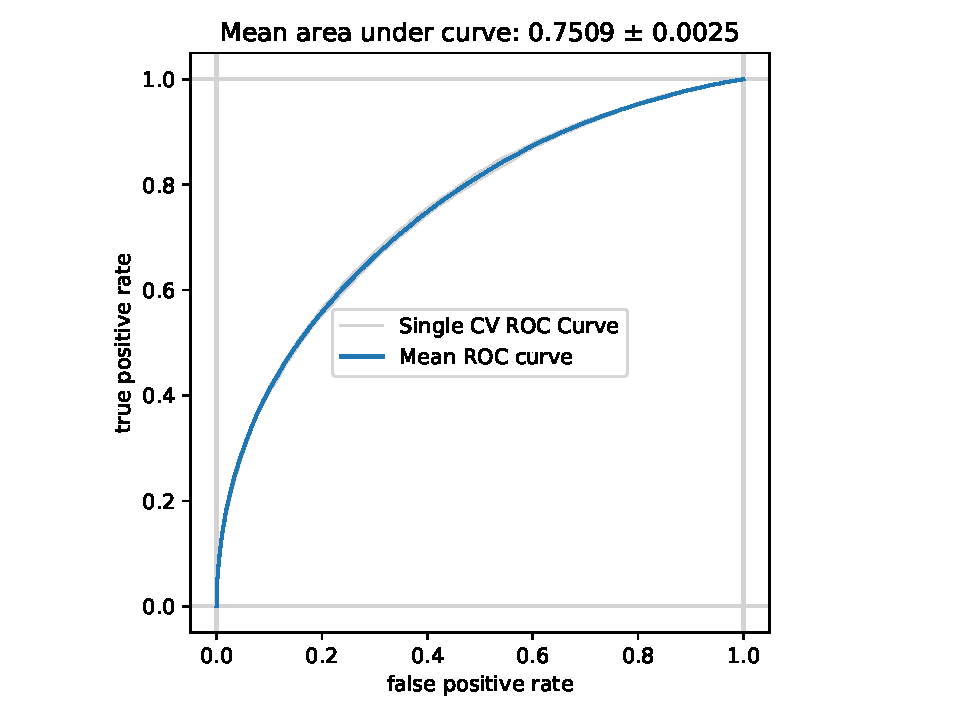
\includegraphics[width=\textwidth]{Plots/data_mc/data_mc_separation.pdf}
  \caption{ROC curve for a random forest model discriminating between proton MC simulations and observed data based in the features implemented in the \texttt{FeatureStream}. The resulting AUC of 0.7509\,\pm\,0.0025 is very high and therefore represents a good discrimination. The proton MC simulations are supposed to model the vast majority of observed data, since the hadron flux is dominating. An AUC this large thus indicates strong data MC mismatches.}
  \label{fig:mcd_roc}
\end{figure}
%

\addtocontents{toc}{\protect\setcounter{tocdepth}{0}}
